\chapter{\label{chap:grundlagen}Grundlagen}
Eine Anwendung, die für den Offline-Gebrauch entwickelt wurde, ist sowohl mit, als auch ohne Internetverbindung vollständig einsatzbereit.\\
Dies erfordert einige Grundvoraussetzungen. Die Daten müssen zuerst auf dem Endgerät gespeichert werden, um offline erreichbar zu sein.
Gibt es eine serverseitige Datenbank, müssen die Daten zwischen Server und Client synchronisiert werden. Ist die Anwendung kollaborativ, muss die Synchronisation zwischen allen Beteiligten stattfinden. Synchronisation erfordert den Umgang mit Konflikten, denn es dürfen auf keinen Fall Daten verloren gehen.\\
Dieses Kapitel beschreibt die grundlegenden Optionen eine Anwendung offlinefähig zu machen, geht im Speziellen auf Konflikte und deren Lösungsstrategien ein. 
%
% Offline-First
%
\section{\label{chap:offlinefirst}Offline First}
Offline First heißt, die Bestandteile einer Anwendung so zu verwalten, dass nach der ersten Verwendung keine Internetverbindung mehr notwendig ist um deren grundlegenden Funktionen zu nutzen.\todo{Quelle}\\
Native \Glspl{App} existieren und funktionieren grundsätzlich solange offline, bis sie versuchen online Daten abzurufen.\\
note{Harte, weiche, mittlere Probleme (verschiedene Stufen von offlinefähig??)}\\

Bei einer bestehenden Internetverbindung ist das Laden der Ressourcen aus dem Cache schneller als aus dem Netz. Daten, die zuerst auf dem Endgerät gespeichert werden, gehen auch bei plötzlichen Verbindungsverlust nicht verloren. \todo{Synchronisation!}\\\\
Dieser Abschnitt zeigt die verschiedenen Möglichkeiten der lokalen Dateinspeicherung und deren Synchronisation mit einer serverseitigen Datenbank auf.
%
% Cache ServiceWorker AppCache
%
\sub{Lokale Speicherung im Cache}
Das Cachen der \gls{Assets} ist der erste Schritt um Daten offline verfügbar zu machen. Browser haben die Möglichkeit, diese Dateien in ihrem Cache zu speichern. Dieser ist nicht persistent, denn sobald der Speicherplatz voll ist werden enthaltene Daten gelöscht~\cite{cache}.
%
% Appcache
%
\subsub{Appcache}
Um mehr Kontrolle darüber zu bekommen, was wann und für wie lange gespeichert werden soll, wurde der Application Cache (AppCache) zur \gls{HTML}-Spezifikation hinzugefügt.
Im Juni 2016\footnote{siehe \url{https://github.com/w3c/html/pull/444/commits}} wurde der AppCache wieder aus den Web-Standards entfernt, und wird nicht mehr empfohlen.
In der Theorie stellte sich der Application Cache als einfach anzuwenden und unproblematisch dar. Um eine webbasierte Anwendung offline auszuliefern wurde benötigte es eine Textdatei -- der \tt{cache manifest}-Datei -- mit der Endung \tt{.appcache}. Dort wurden alle Ressourcen aufgelistet, welche der Browser cachen sollte.
Die Datei wurde dann über das \tt{manifest}-Attribut in die \gls{HTML}-Dateien der Webanwendung eingebunden werden.
%
\lstset{language=HTML,
caption={Beispiel einer \gls{HTML}-Datei mit einer Manifest-Attribut Einbindung},label={code:appcache_html}}
\begin{lstlisting}
  <!DOCTYPE html>
  <html manifest="example.appcache">
    <head>
      <title>Example Application Cache</title>
      <link rel="stylesheet" href="style.css">
      <script src="index.js"></script>
    </head>
    <body>
      ...
    </body>
  </html>
\end{lstlisting}
%
Die über das \tt{manifest}-Attribut eingebundene Cache-Datei kann folgendermaßen aussehen:
\lstset{language=python,
caption={Beispiel einer \normalfont{\tt{.appcache}}\itshape{-Datei}},
label={code:appcache}}
\begin{lstlisting}
  CACHE MANIFEST
  # version comment for triggering updates
  # v1
  style.css
  index.js
  assets/cat.png
\end{lstlisting}
Alle Seiten, mit dem manifest-Attribut und die, die explizit in der Textdatei beschrieben wurden, wurden vom Browser gespeichert~\cite{appcache}.\\
In der Praxis jedoch zeigten sich zahlreiche Probleme mit dem AppCache. So wurde der Application Cache nur aktualisiert wenn sich der Inhalt der des Manifests geändert hat. Dann mussten alle Dateien neu heruntergeladen werden.
Wurden das Manifest und eine andere Datei geändert, wurden die geänderten Dateien nicht unbedingt erneut gespeichert. Denn wenn der Server zusammen mit den Dateien keine Cache-Header sendete, so speicherte der Browser die Datei nach einem Cache-Header-Wert den er `errät`. So konnte es passieren, dass der Browser annahm, eine Datei brauche keine Aktualisierung und weiterhin die alte, gecachte Version auslieferte~\cite{noappcache}.\\
Als Reaktion auf diese Probleme wurde der Service Worker entworfen.
%
% Service Worker
%
\subsub{Service Worker}
Ein Service Worker ist ein Skript, das zwischen Netzwerk und Browser sitzt und von Letzterem im Hintergrund ausgeführt wird. Die Kernfunktion des Service Workers ist es, Netzwerkanfragen abzufangen um sie zu verarbeiten und im Cache zu verwalten~\cite{serviceworker}.\\
Gegenwärtig besitzen -- bis auf den Internet Explorer -- sämtliche Desktop-Browser, und alle gängigen mobilen Browser eine Unterstützung für Service Worker.
%
\begin{figure}[H]
	\centering
	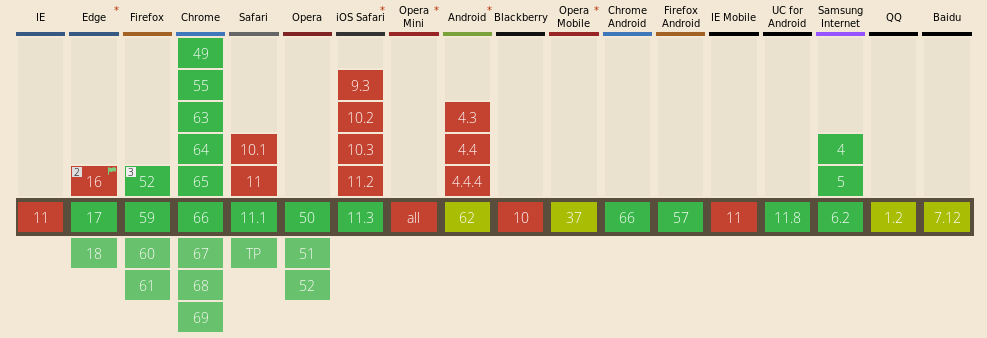
\includegraphics[width=1\textwidth]{ServiceWorker_all}
	\grayRule
	\caption{Browserkompatibilität für Service Worker, Quelle: ~\cite{caniuse-sw}}
	\label{fig:serviceworker}
\end{figure}
%
Mit dem Service Worker können wie mit dem App Cache statische Ressourcen sofort beim ersten Besuch der Seite im Cache gespeichert werden. Es lässt sich hierbei unterscheiden, ob die Daten vor der ersten Verwendung, oder später im Cache gespeichert werden sollen. Für den ersten Fall eignen sich statische Inhalte wie Schriften oder JavaScript--Dateien, für den zweiten größere Ressourcen die nicht sofort benötigt werden.\\
Zusätzlich bietet der Service Worker die Möglichkeit auf Interaktionen zu reagieren. Den NutzerInnen kann angeboten werden bestimmt Inhalte der Seite, wie zum Beispiel ein Video, später, bzw. offline anzuschauen. Diese werden dann im Cache gespeichert und sind somit offline verfügbar.
Service Worker erlauben außerdem den Zugriff auf Push-Benachrichtigungen und das Background Sync \gls{API}. Die Hintergrundsynchronisation kann einmalig oder in festgelegten Intervallen stattfinden und ist besonders für nicht dringende Aktualisierungen wertvoll~\cite{offline_cookbook}.
%
% Browser
%
\sub{Lokale Speicherung im Browser}
Der zweite Schritt Daten offline verfügbar zu machen ist sie im Browser zu speichern. Einige Konzepte hierfür werden im Folgenden erläutert.
%
\subsub{Web Storage}
Das Web Storage \gls{API} ist ein Web-Standard mit dessen Hilfe Daten als Schlüssel / Wert Paare im Browser gespeichert werden können. Es wird, wie Abbildung \ref{fig:webStorage} zeigt, von allen relevanten Browsern unterstützt.
Web Storage umfasst zwei Mechanismen. Den Session Storage und den Local Storage.\\
Der Session Storage existiert nur so lange der Browser geöffnet ist.
Das heißt alle Daten die im Session Storage gespeichert werden, existieren nicht mehr sobald der Browser geschlossen wird. Daten die im Local Storage gespeichert sind, existieren dort solange bis der Browser Cache geleert wird~\cite{webstorage}.
\begin{figure}[H]
	\centering
	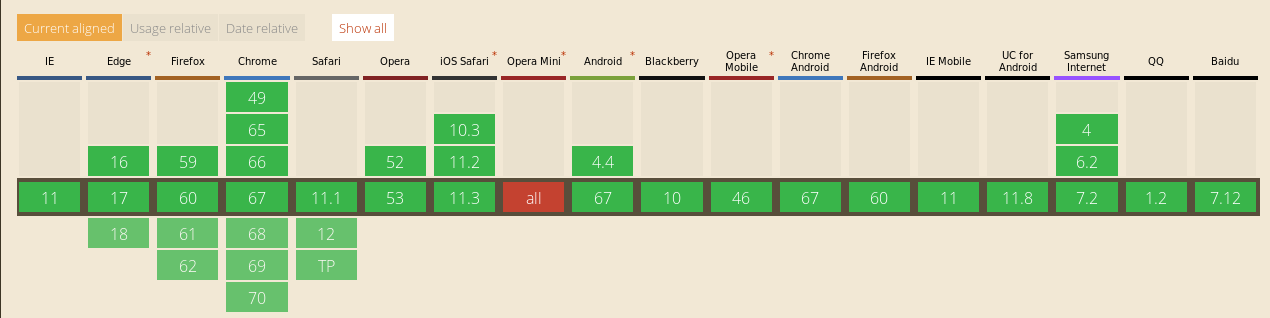
\includegraphics[width=\textwidth]{webStorage}
	\grayRule
	\caption{Browserkompatibilität für Web Storage, Quelle: ~\cite{caniuse-ws}}
	\label{fig:webStorage}
\end{figure}
Der von den Browsern freigegebene Cache-Space für Web Storage variiert, ist aber meist auf 10 MB begrenzt. Der größte Nachteil ist wohl, dass Web Storage synchron arbeitet und so andere Operationen, wie zum Beispiel das Rendern der Seite, blockieren kann~\cite{webstorage-con}.
%
%
\subsub{Web SQL}
Eine andere der lokalen Speicherung im Browser ist die Web SQL Datenbank.
Sie hat ein asynchrones \gls{API} und unterstützt die grundlegenden SQL Abfragen. Web SQL sollte in den W3C Standards aufgenommen werden. Aus Mangel unabhängigen Implementierungen wie eine andere \gls{DB} als SQLite im Backend wurde es abgelehnt~\cite{websql}.\\
Das Web SQL \gls{API} wird nur von den Webkit--Browsern unterstützt. Also nicht von Firefox, dem Internet Explorer oder dessen neueren Variante Edge~\cite{caniuse-websql}.
%
%
\subsub{IndexedDB}
IndexedDB ist eine weitere Variante der clientseitigen Datenspeicherung. Die auf Java"-Script basierende, objektorientierte Datenbank erlaubt neben dem Speichern von größeren Datenmengen in Form von Objekten auch das Speichern von Dateien. Durch die Verwendung von Indizes lassen sich Objekte schnell speichern und finden. Das asynchrone \gls{API} erlauben Datenbankabfragen die keinen anderen Prozess blockieren~\cite{idb}.
\begin{figure}[H]
	\centering
	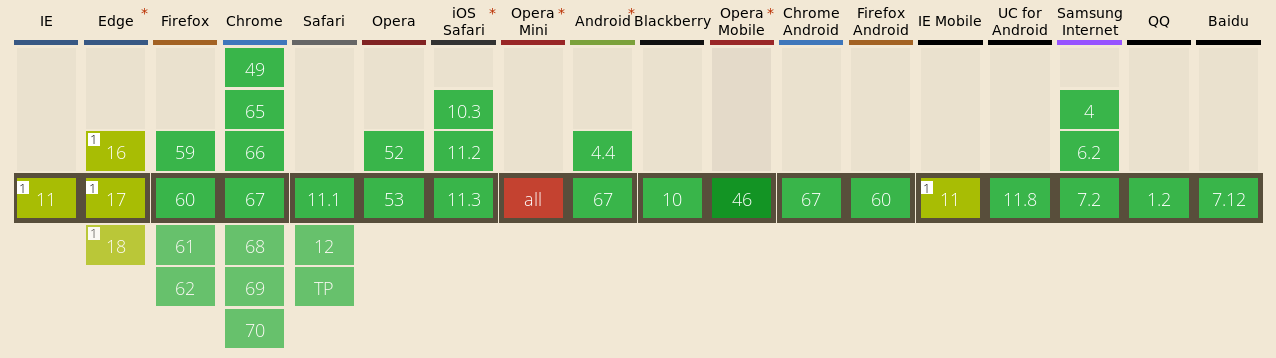
\includegraphics[width=\textwidth]{indexedDB}
	\grayRule
	\caption{Browserkompatibilität für IndexedDB, Quelle: ~\cite{caniuse-idb}}
	\label{fig:indexedDB}
\end{figure}
Wie in Abbildung \ref{fig:indexedDB} zu sehen ist, wird IndexedDB von allen gängigen Browsern unterstützt. 
%
\subsub{IndexedDB 2.0}
Im Januar 2018 wurde die zweite Version des IndexedDB \glspl{API} zur W3C Spezifikation hinzugefügt. Es erweitert die erste Verion um Funktionalität und verbessert die Performance~\cite{idb2}.
Die Aktualität dieser Spezifikation spiegelt sich in der Browserunterstützung wider. Die Abbilung \ref{fig:indexedDB2} zeigt, dass die zweite Version nur von den beliebten \highlight{(haha)} Desktopbrowsern und einigen mobilen Browsern unterstützt wird. 
\begin{figure}[H]
	\centering
	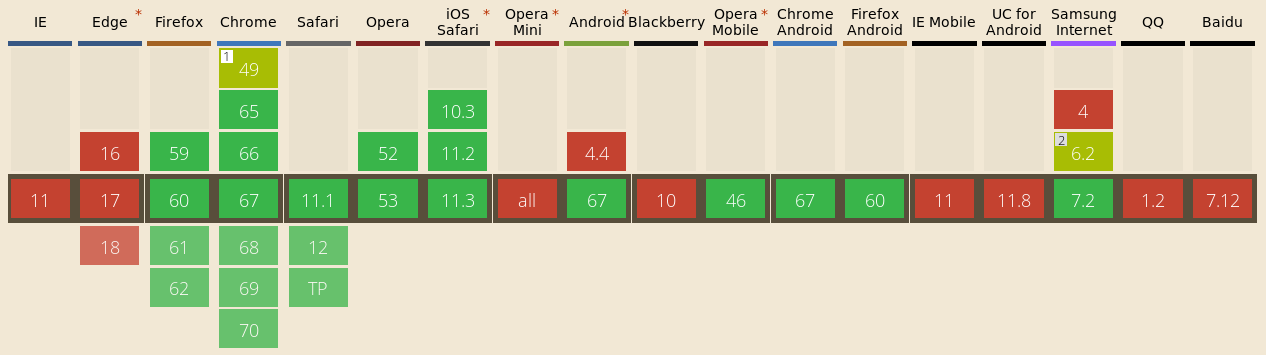
\includegraphics[width=\textwidth]{indexedDB2}
	\grayRule
	\caption{Browserkompatibilität für IndexedDB 2.0, Quelle: ~\cite{caniuse-idb}}
	\label{fig:indexedDB2}
\end{figure}
IndexedDB wird stetig weiterentwickelt und es gibt bereits einen Spezifikationsentwurf für die dritte Version~\cite{idb3}. 
%
% Sync
%
\sub{Datenbanksynchronisation}
Im Allgemeinen ist ein Synchronisationsprotokoll die Möglichkeit für zwei Partenen, beispielsweise Client und Server, den Zustand voneinander zu kennen. Der Client schickt seine Daten an den Server und umgekehrt, Konflikte werden gelöst, solange bis beide Parteien denselben Zustand haben.
Leider sind Synchronisationsprotokolle schwer zu implementieren und führen häufig zu einem frustrierenden Ergebnis: Dokumente oder Fotos werden nicht repliziert, es gibt doppelte oder verlorene Daten und alle möglichen Arten von Fehlverhalten bei kollaborativen Anwendungen.\\
CouchDB hat ein intergiertes \hyperref[sec:replication]{Replikationsprotokoll}, das diesen Teil behandelt.  
%
% Couch
%
\subsub{\label{sec:couch}CouchDB}
Apache CouchDB\tm ist ein \gls{DBMS} das seit 2005 als freie Software entwickelt wird. Die dokumentenorientierte \gls{DB} funktioniert sowohl als einzelne Instanz, als auch im Cluster, in dem ein Datenbanksserver auf einer beliebig großen Anzahl an Servern oder Virtuellen Masschinen ausgeführt werden kann.\\
% So kann die Datenschicht beliebig skaliert werden, um die Anforderungen vieler BenutzerInnen zu erfüllen.
CouchDB verwendet das \gls{HTTP}--Protokoll und \gls{JSON} als Datenformat, weswegen es mit jeder Webfähigen Anwendung kompatibel ist. CouchDB wird über ein \gls{REST}ful \gls{HTTP} \gls{API} angesprochen. So können Daten über die für den \gls{REST}ful Services standardisierten Methoden wie zum Beispiel GET, POST, PUT, DELETE abgerufen oder manipuliert werden.\\\\
Das implementierte Replikationsmodell erlaubt die Synchronisation bzw. bidirektionale Replikation zu verschiedenen Geräten, was das besondere Merkmal von CouchDB ist. 
Die genaue Funktionsweise des Protokolls wird in \autoref{sec:replication} detailliert beschrieben.\\
Dieses Protokoll ist die Grundlage für Offline First Anwendungen.
Dank des Replikations--\gls{API} kann kann sich eine CouchDB kontinuierlich und eigenständig mit einer anderen Datenbank die dasselbe Protokoll implementiert, synchronisieren.
Wenn Konflikte auftreten, beispielsweise durch gleichzeitiges Bearbeiten eines Dokuments von zwei Personen ohne Netzwerkverbindung, werden diese als solche markiert, jedoch nicht von selbst aufgelöst~\cite{couch}. Die Lösung der Konflikte muss in der Anwendung implementiert sein.
So kann gewährleistet werden, dass keinerlei Daten verloren gehen.\\\\
CouchDB ist für Server konzipiert. Für Browser gibt es \hyperref[sub:pouch]{PouchDB} und für native iOS- und Android--\glspl{App} wurde Couchbase Lite entwickelt.
Des Weiteren gibt es noch die Datenbanken Couchbase und Cloudant.
Alle verwenden das CouchDB Replikationsprotokoll und können Daten miteinander replizieren und~\cite{couch}.
%
% Pouch
%
\subsub{\label{sub:pouch}PouchDB}
Als Ergänzung zu CouchDB kann PouchDB verwendet werden. PouchDB ist die Java"-Script Implementierung von CouchDB.
Sie ist quelloffen und wurde so konzipiert, dass sie in allen modernen Browsers läuft. Dort ermöglicht PouchDB es Daten zu persistieren, sodass sowohl offline als auch online verfügbar sind.
PouchDB speichert die Daten in IndexedDB und stellt für das Abrufen und Manipulieren derer ein einheitliches \gls{API} zur Verfügung.\\
Sind die Daten einmal offline gespeichert können sie, dank des CouchDB Replikationsprotokolls, sobald die Awendung wieder online ist mit CouchDB kompatiblen Servern synchronisiert werden~\cite{pouch}.
% %
% % PWA
% %
% \sub{\label{sub:pwa}Progressive Web Apps \todo{raus?}}
% \Gls{PWA} ist eine Bezeichnung für eine mobil nutzbare Webseite, die eine Brücke zwischen der nativen
% Applikation und einer Webseite schlägt.
% Der Begriff \gls{PWA} wurde im Jahr 2015  von Alex Russel und seiner Frau Frances Berriman geprägt.
% Dieser beschreibt Webseiten, die die positiven Funktionen von nativen Applikationen mitbringen, aber statt über App Stores installiert zu werden, im Webbrowser existieren. Die Webseiteninhalte sind ohne die Installation sofort und jederzeit für die NutzerInnen abrufbar. Schon beim zweiten Besuch der Webseite ist die Ladezeit der Daten verkürzt und sie ist offline, oder auch bei schlechter Internetverbindung nutzbar. Nach mehrmaligem Aufruf kann die \gls{PWA} über den Browser installiert und zum Startbildschirm hinzugefügt werden. Russel und Berriman legen folgende Einenschaften einer \gls{PWA} fest:
% \begin{itemize}
% 	\item Responsive %to fit any form factor
% 	\item Connectivity independen]% Progressively-enhanced with Service Workers to let them work offline
% 	\item App-like-interaction]% Adopt a Shell + Content application model to create appy navigations \& interactions
% 	\item Fresh %Transparently always up-to-date thanks to the Service Worker update process
% 	\item Safe %Served via TLS (a Service Worker requirement) to prevent snooping
% 	\item Discoverable %Are identifiable as “applications” thanks to W3C Manifests and Service Worker registration scope a llowing search engines to find them
% 	\item Re-engageable %Can access the re-engagement UIs of the OS; e.g. Push Notifications
% 	\item Installable %to the home screen through browser-provided prompts, allowing users to “keep” apps they find most useful without the hassle of an app store
% 	\item Linkable %meaning they’re zero-friction, zero-install, and easy to share. The social power of URLs matters.
% \end{itemize}
% \todo{Näher erläutern?}~\cite{pwa}.

%
% Konflikte
%
% 1. Definition
Als Konflikt wird die Situation bezeichnet, in der verschiedene Versionen des gleichen Dokuments auf mehreren Geräten oder Datenbanken gespeichert sind (vgl. ~\cite{couchDB} S. 153).
Konflikte gehören in verteilten Systemen zur Realität und lassen sich nicht vermeiden.
Ein verteiltes System ist per Definition ein Zusammenschluss unabhängiger Computer, die sich für die NutzerInnen als ein einziges System präsentieren (vgl. ~\cite{tanenbaum} S. 2).
Einfacher gesagt, besteht ein verteiltes System, sobald zwei oder mehrere Computer über das Netzwerk miteinander verbunden sind.
Die spezielle Eigenschaft von Netzwerken ist jedoch, dass die Verbindung jederzeit abbrechen kann.
Gareth Wilson beschreibt in seinem Artikel die acht Irrtümer zur verteilten Datenverarbeitung ~\cite{fallacies}:
\begin{enumerate}
  \item Das Netzwerk ist zuverlässig
  \item Die \gls{Latenz}zeit ist gleich null
  \item Die Bandbreite ist unendlich
  \item Das Netzwerk ist (informations)sicher
  \item Die Netzwerkstruktur wird sich nicht ändern
  \item Es gibt eineN AdministratorIn
  \item Die Datentransportkosten sind gleich null
  \item Das Netzwerk ist homogen
\end{enumerate}
Aus diesen irrtümlichen Annahmen über das Netzwerk ergeben sich Fehlerszenarien. So kann es passieren, dass der zweite Computer entweder sehr weit entfernt, sehr beschäftigt oder ausgeschaltet ist. Diese Fehlerszenarien können dazu führen, dass ein Konflikt entsteht.
Anhand des folgenden Beispiels wird ein mögliches Fehlerszenario für den Fall des unzuverlässigen Netzwerks aufgegriffen.\\
%
Zwei Personen treffen sich im Zug und verstehen sich auf Anhieb sehr gut. Person A, nennen wir sie Amilia, gibt Person B, nennen wir sie Rory, ihre Telefonnummer. Der Zug fährt durch einen Tunnel und das Netzwerk bricht ab, als Rory Amilias Nummer in sein Adressbuch, das in Form einer \gls{App} auf seinem Laptop gespeichert ist, schreibt.
Amilia diktiert ihre Telefonnummer falsch, mit einem Zahlendreher, weil sie die Nummer noch nicht lange hat.
Zur Sicherheit schickt Amilia Rory ihre Nummer zusätzlich per E-Mail. Rory schaltet seinen Laptop aus, weil er sich mit Amilia unterhalten möchte.
Am Abend ist Rory zu Hause angekommen und er speichert Amilias Nummer aus der E-Mail in seinem Adressbuch auf seinem stationären Desktop PC.
Jetzt gibt es Amilias Telefonnummer mit unterschiedlichen Informationen in Rorys Adressbuch auf verschiedenen Geräten.
Wenn Rory am nächsten Tag seinen Laptop startet und das Adressbuch sich mit dem auf dem PC synchronisiert, entsteht ein Konflikt.
Es gibt zwei unterschiedliche Versionen von Amilias Telefonnummer auf Rorys Geräten.\\\\
% Die korrekte Telefonnummer vom stationären PC befindet sich bereits auf dem Server und wird nun, da sich jetzt das Adressbuch auf dem Laptop mit dem Server synchronisiert, von der Nummer mit dem Zahlendreher überschrieben.
% Die falsche Telefonnummer wird gespeichert und die richtige ist verloren.\\\\
%
%
Konflikte sind in zwei Kategorien einzuteilen. Es gibt solche, die vom System selbst gelöst werden können und solche, die eine spezielle Behandlung brauchen.
Gibt es eine gleichzeitige Änderung an unterschiedlichen Stellen eines Dokuments, muss das kein Problem darstellen.
Das Dokument kann beide Aktualisierungen erhalten, indem die Änderungen zusammengefügt werden.
Diese Prozedur wird \it{merge} genannt und ist durch Systeme wie Git\footnote{git steht unter \url{https://git-scm.com/downloads} zum Download bereit}, einer Software zur verteilten Versionsverwaltung, den meisten EntwicklerInnnen bekannt. Diese Art Konflikt kann selbstständig vom System gelöst werden.\\

Die Konflikte, die durch verschiedene Änderungen an ein und derselben Stelle des Dokuments entstehen, benötigen eine aufwändigere Behandlung.
Es muss festgestellt werden, welche Version die korrekte ist und gespeichert werden soll.
Die Wiederherstellung der Datenkonsistenz bei Konflikten kann dazu führen, dass einige oder alle Aktualisierungen ganz oder teilweise gelöscht werden.
Zur Lösung dieses Problems wurden verschiedene Managementstrategien entworfen, die im Folgenden vorgestellt werden.
%
%
% \begin{description}[leftmargin=0.5cm,style=nextline]
% 	\item[1. Das Netzwerk ist zuverlässig] ~ Der Strom kann ausfallen oder Glasfaserkabel können kaputt sein --- Das Netzwerk ist nicht zuverlässig.
% 	\item[2. Die \gls{Latenz} ist gleich null] ~ Glasfaserkabel werden durch Mikrowellen (oder andere Technologien) ersetzt um Millisekunden an Zeit zu sparen. Das würde nicht passieren, wäre die \gls{Latenz} bei null. Es dauert nun mal eine gewisse Zeit(ms) wenn ein Signal eine (geografisch)weite Strecke zurücklegen muss --- Die Latenz ist nicht gleich null.
% 	\item[3. Die \gls{Bandbreite} ist unendlich] ~ Daten können nicht schneller fließen als die Komponenten die sie verarbeiten (\gls{Middleware}, Datenbank \ldots) --- Die Bandbreite ist nicht unendlich.
% 	\item[4. Das Netzwerk ist sicher] ~ Der \sc{Heartbeat-bug}\footnote{\url{http://heartbleed.com/} -- Zugriff: 07.04.2018}, der im Jahr 2014 behoben wurde und die Sicherheitslücke im ICE-\gls{WLAN} im Jahr 2016\footnote{\url{https://netzpolitik.org/2016/datenschutz-im-zug-deutsche-bahn-will-sicherheitsluecke-in-neuem-ice-wlan-schliessen/} -- Zugriff: 07.04.2018} sind nur zwei Beispiele die zeigen, dass das Netzwerk nicht sicher ist.
% 	\item[5. Die Netzwerkstruktur wird sich nicht ändern] ~ Eine Datenbank kann beispielsweise über mehrere Server verteilt sein, die (teilweise) voneinander abhängig sind. Ein Server mit Abhängigkeiten kann ausfallen, es kann eine Aktualisierung für einen anderen Server geben --- die Struktur ändert sich.
% 	\item[5. Die Netzwerkstruktur wird sich nicht ändern] ~ Eine Datenbank kann beispielsweise über mehrere Server verteilt sein, die (teilweise) voneinander abhängig sind. Ein Server mit Abhängigkeiten kann ausfallen, es kann eine Aktualisierung für einen anderen Server geben --- die Struktur ändert sich.
% 	\item[6. Es gibt eineN AdministratorIn] ~ Es kann beliebig viele AdministratorInnen geben.
% 	\item[7. Die Datentransportkosten sind gleich null] ~ Netflix bezahlte anfang 2014 diversen InternetanbieterInnen dafür, dass Netflix KundInnen bevorzugten Internetzugang haben.
% 	\item[8. Das Netzwerk ist homogen] ~ Es gibt verschiedene Arten von Netzwer: 3G, 4G, LTE, WiFi. Wird beeinflusst durch Hardware (Smartphone, Tablet, PC, Laptop, Router \ldots)~\cite{fallacies}
% \end{description}
